\documentclass{beamer}

% Theme and color settings
\usetheme{Madrid}          % Clean, minimal theme
\usecolortheme{default}    % Simple color scheme

% Packages
\usepackage{graphicx}      % For images
\usepackage{amsmath}       % For math support
\usepackage{hyperref}      % For clickable links
% ...existing code...
\usepackage{listings}
\usepackage{xcolor}
\colorlet{punct}{red!60!black}
\definecolor{background}{HTML}{EEEEEE}
\definecolor{delim}{RGB}{20,105,176}
\colorlet{numb}{magenta!60!black}

\lstdefinelanguage{json}{
    basicstyle=\tiny\ttfamily,
    numbers=left,
    numberstyle=\scriptsize,
    stepnumber=1,
    numbersep=2pt,
    showstringspaces=false,
    breaklines=true,
    frame=lines,
    backgroundcolor=\color{background},
    literate=
     *{0}{{{\color{numb}0}}}{1}
      {1}{{{\color{numb}1}}}{1}
      {2}{{{\color{numb}2}}}{1}
      {3}{{{\color{numb}3}}}{1}
      {4}{{{\color{numb}4}}}{1}
      {5}{{{\color{numb}5}}}{1}
      {6}{{{\color{numb}6}}}{1}
      {7}{{{\color{numb}7}}}{1}
      {8}{{{\color{numb}8}}}{1}
      {9}{{{\color{numb}9}}}{1}
      {:}{{{\color{punct}{:}}}}{1}
      {,}{{{\color{punct}{,}}}}{1}
      {\{}{{{\color{delim}{\{}}}}{1}
      {\}}{{{\color{delim}{\}}}}}{1}
      {[}{{{\color{delim}{[}}}}{1}
      {]}{{{\color{delim}{]}}}}{1},
}

% Title, author, date
\title{Pero si mi codigo corre en mi compu!}
\subtitle{Desarollo en Contenedores}
\author{Teresa Bracahamonte \& Nicolas Vega}
\date{\today}

\begin{document}

% Title slide
\begin{frame}
  \titlepage
\end{frame}

\begin{frame}{Acerca de}
  \begin{itemize}
    \item \textbf{Doctora Teresa Bracahamonte:} Experta "Data Scientist" ))
    \item \textbf{Nicolas Vega:} Ingeniero en Informática egresado universidad de Santiago, programador con mas de 15 años de experiencia en desarrollo de software.
  \end{itemize}
\end{frame}

% Table of contents
\begin{frame}{Agenda}
  \tableofcontents
\end{frame}

% Section 1
\section{Introduccion}
\subsection{Que son los entornos de desarrollo en contenedores?}
\begin{frame}{\subsecname}
  Los dev containers permiten tener un ambiente aislado con una serie de configuraciones 
  y features que ayudan a los desarolladores a correr sus aplicaciones mejorando la 
  integracion continua y testing.
  \begin{block}{En estos contenedores encontramos}
    \begin{itemize}
      \item Sistema operativo reducido (\textbf{imagen})
      \item Paquetes de ejecución y productividad (\textbf{features})
      \item Sistema de archivos locales del contenedor
      \item Nuestro código (\textbf{volumen} host:contenedor)
      \item Backend de nuestro IDE 
      \item Pueden correr en entornos locales o remotos
    \end{itemize}
  \end{block}
\end{frame}

\begin{frame}{Detras de la caja negra}
  \begin{figure}
    \centering
    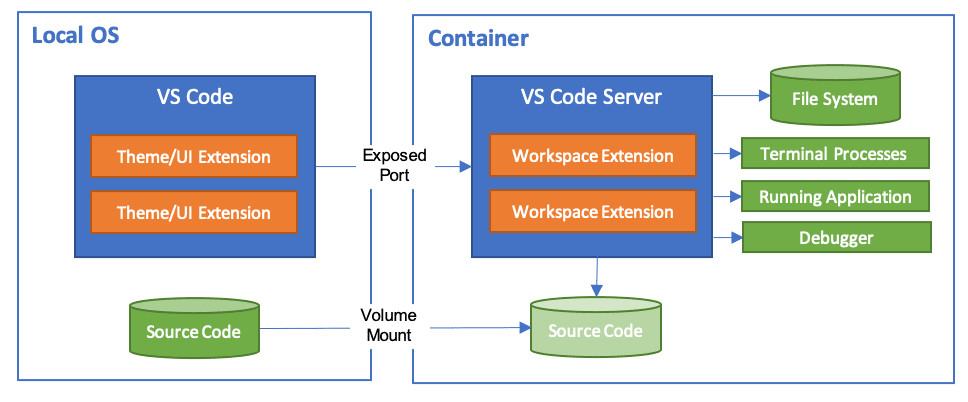
\includegraphics[width=\textwidth]{images/architecture-containers.png}
    \caption{Arquitectura de contenedores en entornos de desarrollo.}
  \end{figure}
\end{frame}

\subsection{Beneficios y Desafios}
\begin{frame}{Beneficios del desarrollo en contenedores}
  \begin{itemize}
    \item \textbf{Aislamiento:} Cada proyecto puede tener su propio contenedor, lo cual previene conflictos entre diferentes versiones de dependencias en proyectos diferentes.
    \item \textbf{Portabilidad:} Funciona en cualquier máquina con Docker.
    \item \textbf{Consistencia:} Contenedores logran encapsular el entorno de desarrollo (librerías, dependencias, etc). Los desarrolladores logran un entorno de desarrollo consistente en todas sus máquinas locales.
    \item \textbf{Facilidad de uso:} Configuración rápida y sencilla.
  \end{itemize}
\end{frame}

\begin{frame}{Desafios asociados al desarollo en contenedores}
  \begin{itemize}
    \item \textbf{Curva de aprendizaje:} Requiere un conocimiento básico, comandos y herramientas relacionadas a contenedores. Esto podría volver lenta la adopción y aumentar la curva de aprendizaje de los desarrolladores.
    \item \textbf{Rendimiento:} El correr los contenedores en local requiere mayor utilización de memoria y CPU, sumado a que se pueden correr múltiples entornos de desarrollo a la vez.
    \item \textbf{Depuración:} Herramientas de depuración pueden ser limitadas.
    \item \textbf{Seguridad:} Los contenedores podrían tener vulnerabilidades o librerías desactualizadas.
  \end{itemize}
\end{frame}
\subsection{Ciclo de desarrollo ideal}
\begin{frame}{\subsecname}
  \begin{figure}
    \centering
    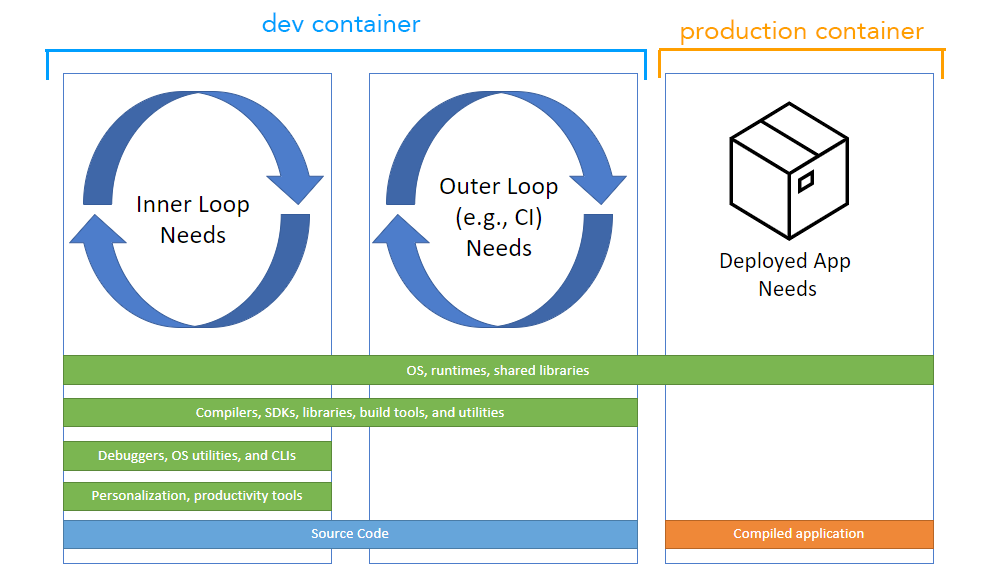
\includegraphics[width=\textwidth]{images/dev-container-stages.png}
    \caption{Dev,CI y Prod}
  \end{figure}
\end{frame}

\section{Setup Inicial}
\begin{frame}{Desarrollo local}
  \begin{block}{Docker}
    \begin{itemize}
      \item \textbf{Docker Desktop:} Herramienta de Docker para correr contenedores en local.
      \item \textbf{Docker CLI:} Interfaz de línea de comandos para interactuar con Docker.
    \end{itemize}
  \end{block}
  \begin{block}{Visual Studio Code}
    \begin{itemize}
      \item \textbf{Dev Containers:} Extensión de Visual Studio Code que permite crear y administrar contenedores de desarrollo.
      \item \textbf{Remote - SSH:} Extensión de Visual Studio Code que permite conectarse a máquinas remotas a través de SSH.
      \item \textbf{WSL:} Extensión de Visual Studio Code que permite trabajar con el Subsistema de Windows para Linux.
    \end{itemize}
  \end{block}
\end{frame}


\subsection{Python uv fastapi en entorno local}
\begin{frame}{\subsecname}
  \begin{columns}
    \begin{column}{0.7\textwidth}
      \begin{itemize}
        \small
        \item Obtener el proyecto desde github
        \item \href{https://github.com/copernicus231/devcontainer-boilerplate-python-uv-fastapi.git}{https://github.com/copernicus231/devcontainer-boilerplate-python-uv-fastapi.git}
        \item Ir a la paleta de comandos y buscar "Dev Containers: Reopen in Container"
        \item Seleccionar "Reopen in Container"
        \normalsize    \end{itemize}
      El contenedor se creara usando el archivo en \textbf{.devcontainer/devcontainer.json}
    \end{column}
    \begin{column}{0.3\textwidth}
      \begin{figure}
        \centering
        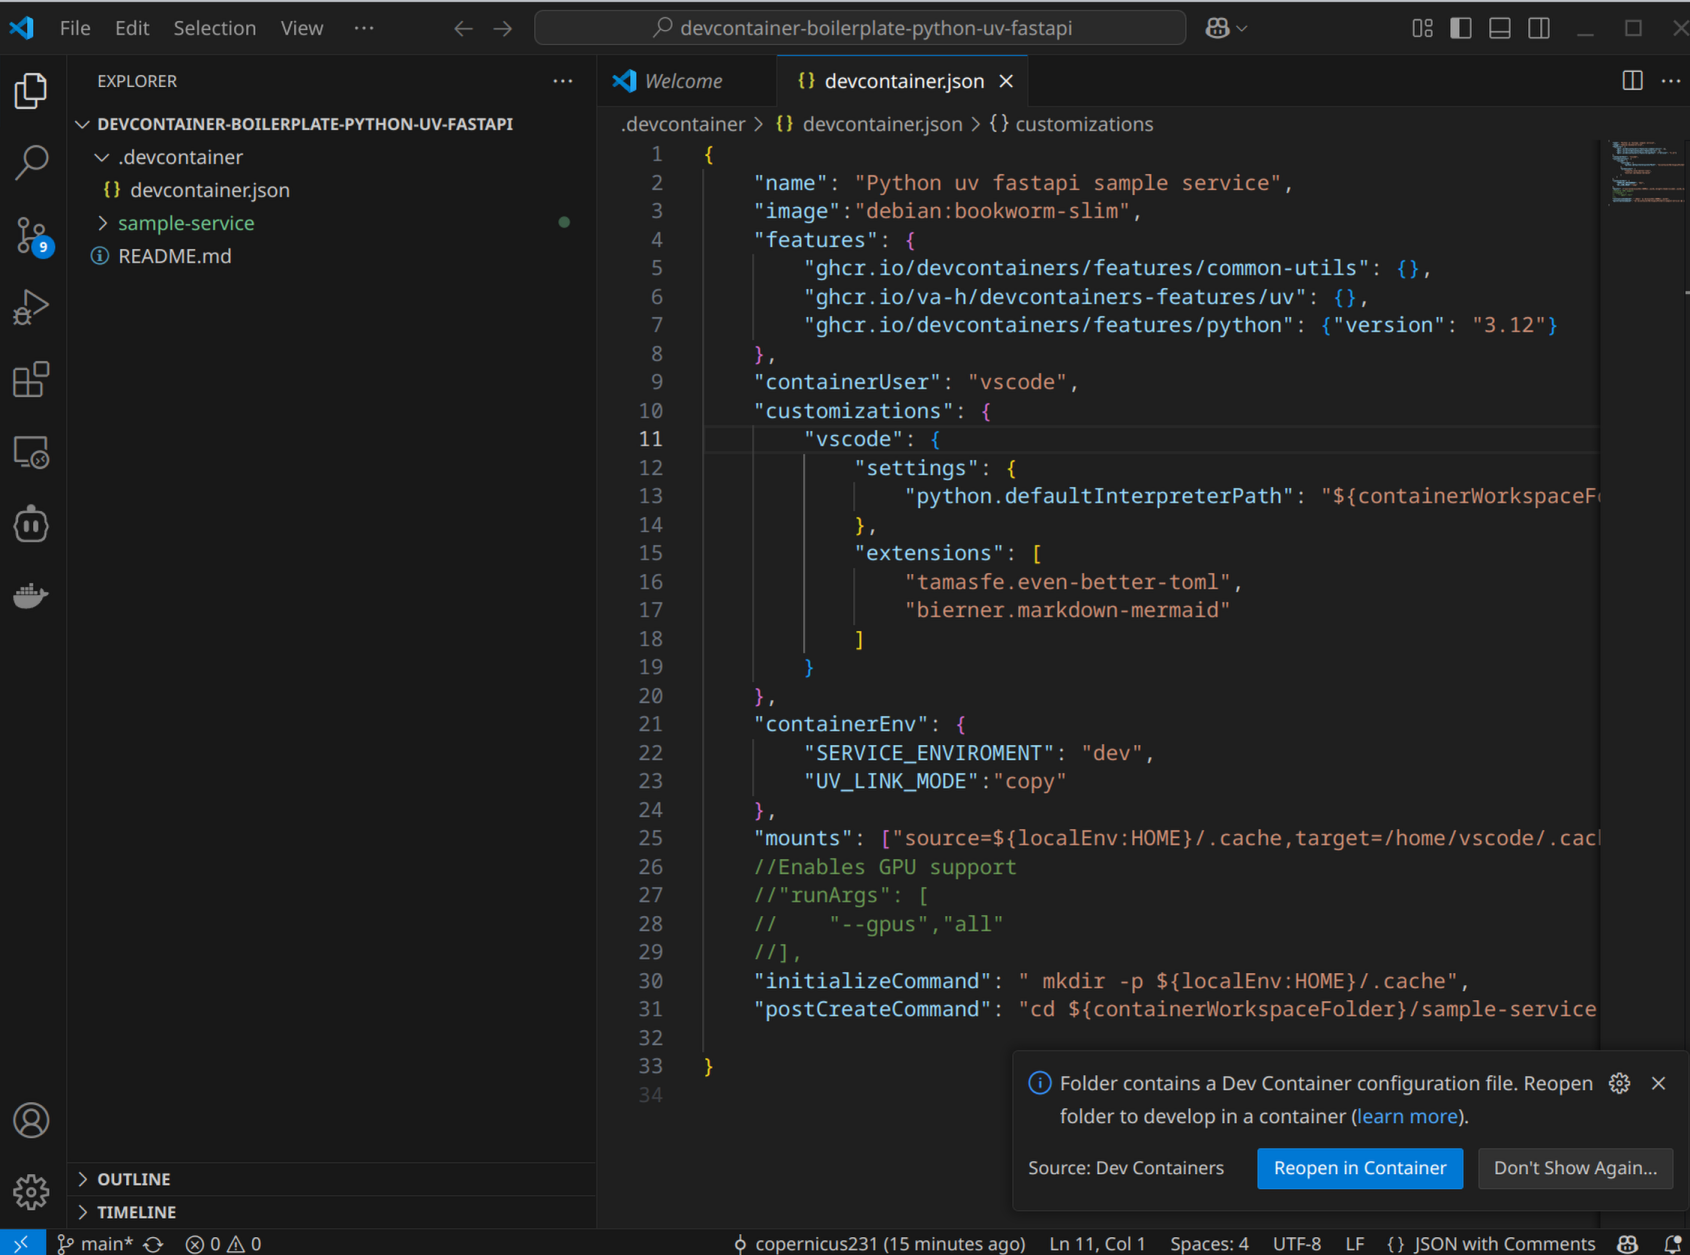
\includegraphics[width=\textwidth]{images/open-container.png}
        \caption{Configuración de FastAPI en contenedor.}
      \end{figure}
    \end{column}
  \end{columns}
\end{frame}


\begin{frame}{\subsecname}
  \begin{columns}
    \begin{column}{0.5\textwidth}
      \begin{itemize}
        \item \texttt{cd simple-service}
        \item \texttt{uv run fastapi dev src/simple\_service/base.py}
      \end{itemize}
        \end{column}
        \begin{column}{0.5\textwidth}
      \begin{figure}
        \centering
        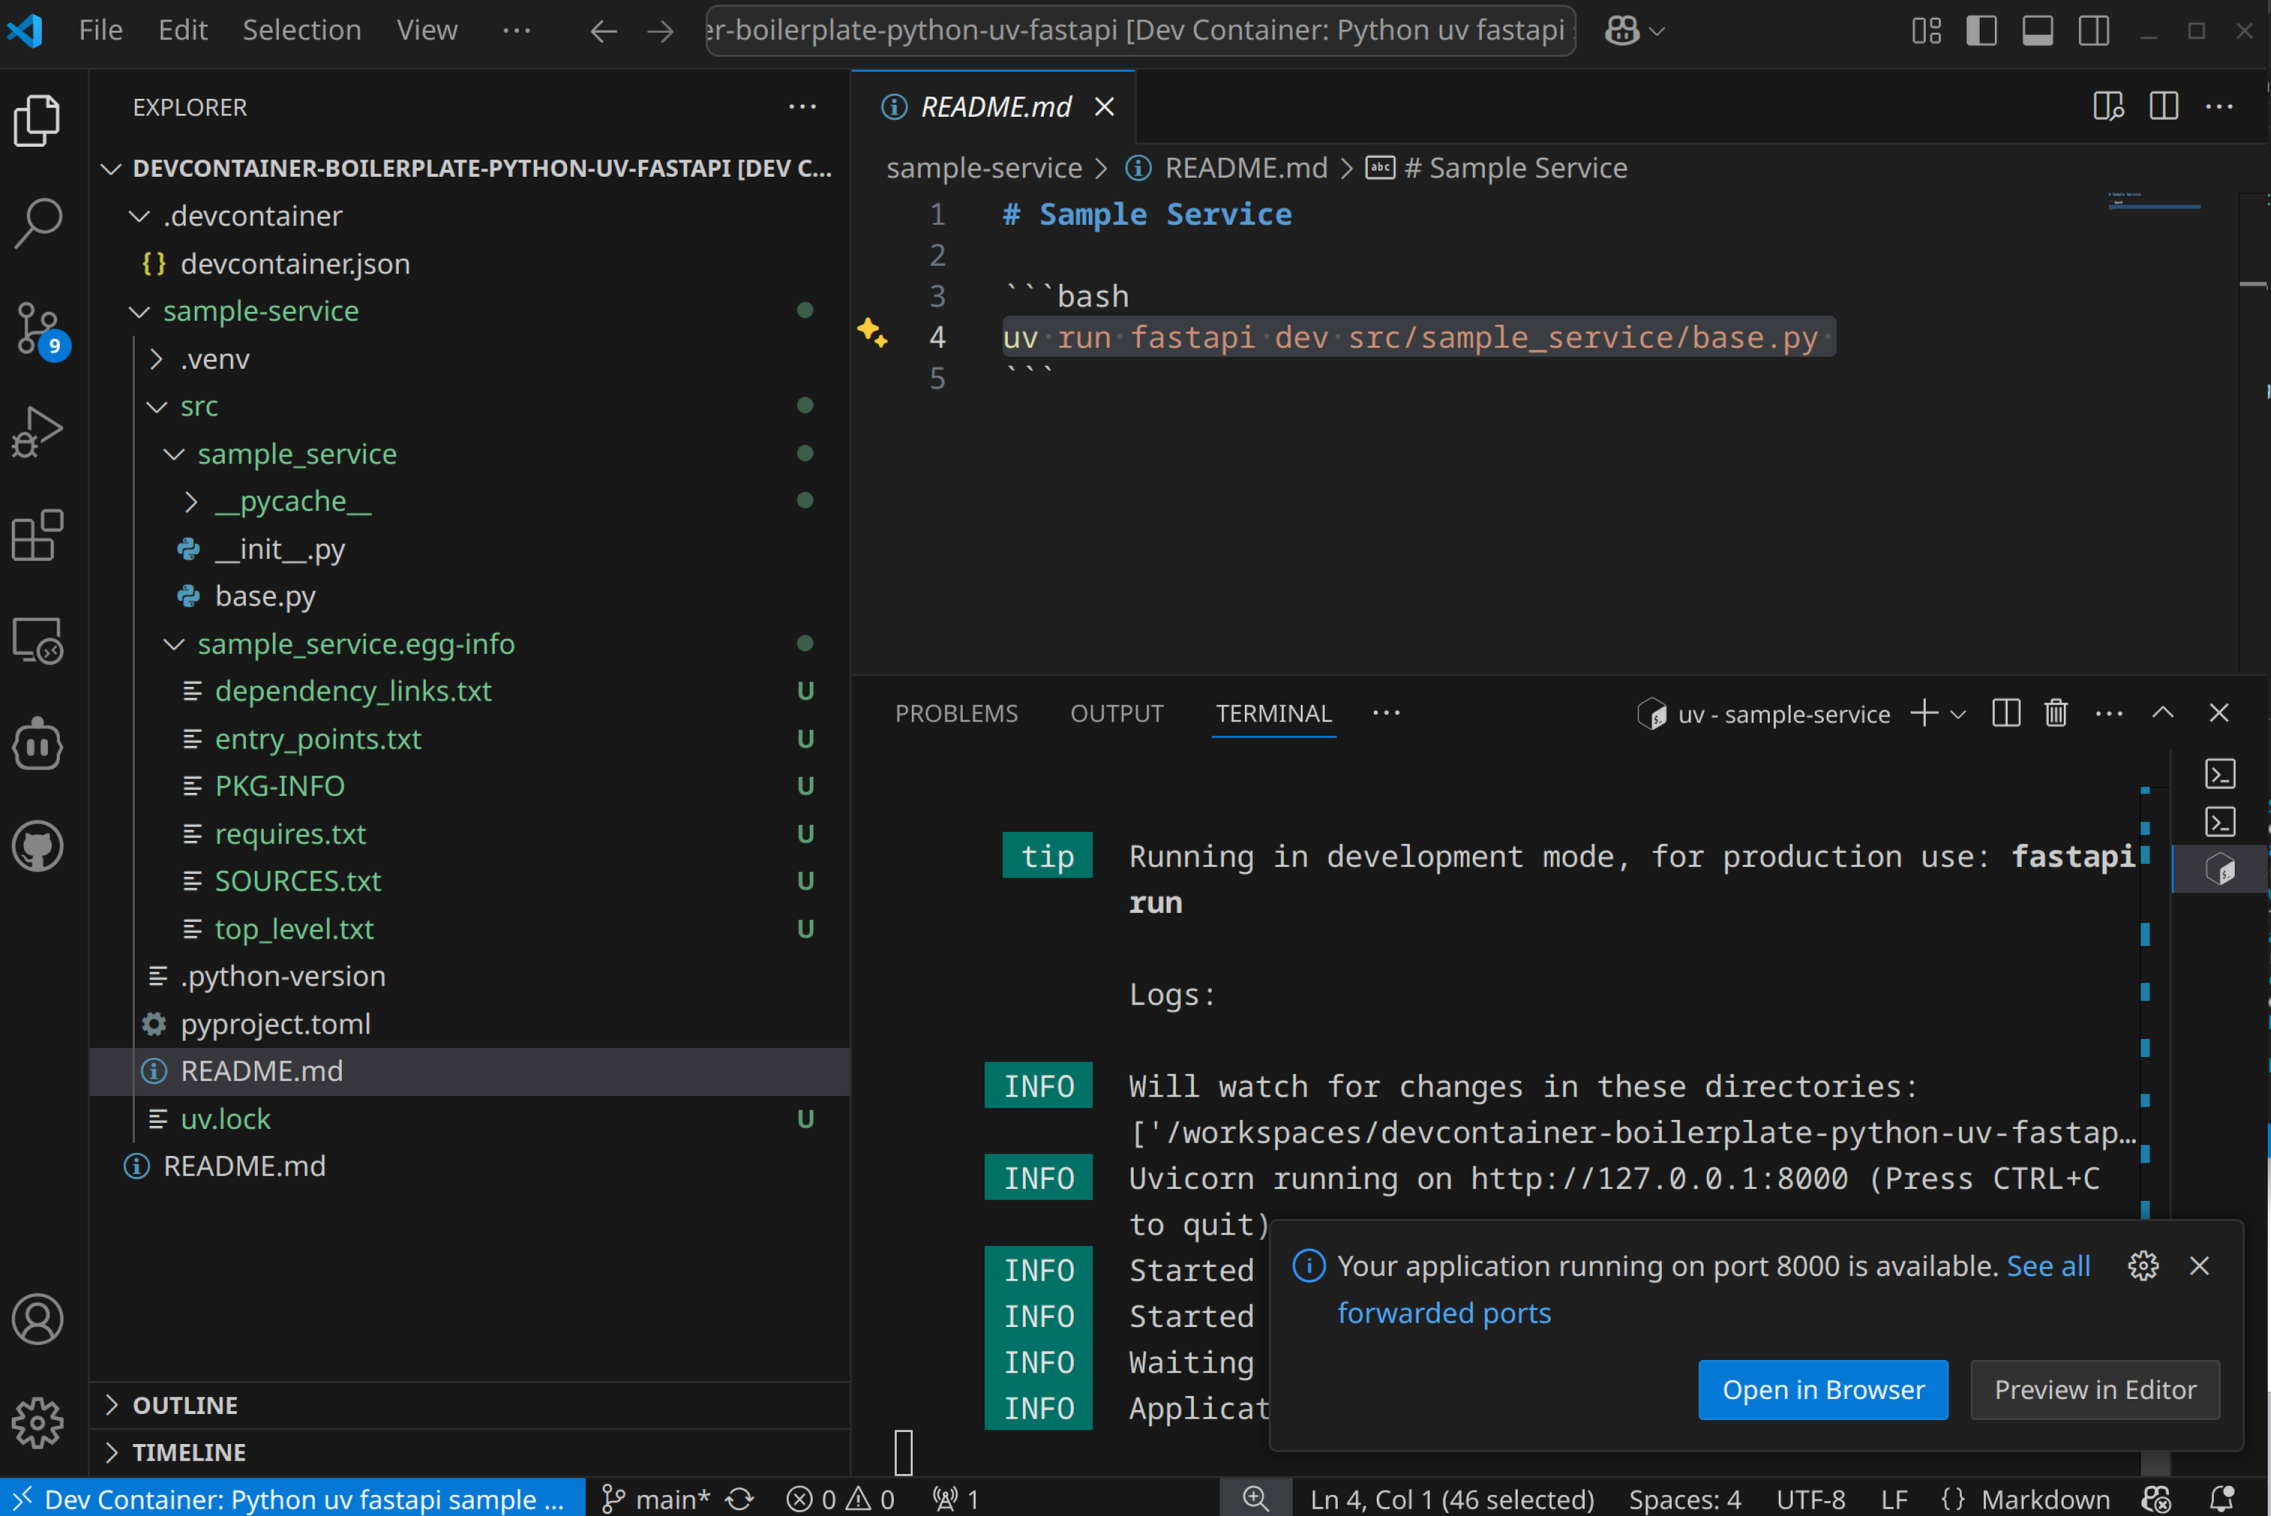
\includegraphics[width=\textwidth]{images/run-fastapi.png}
        \caption{Run fastapi endpoint}
      \end{figure}
        \end{column}
  \end{columns}
\end{frame}
\subsection{Python uv fastapi en Codespaces}
\begin{frame}{\subsecname}
      \begin{figure}
        \centering
        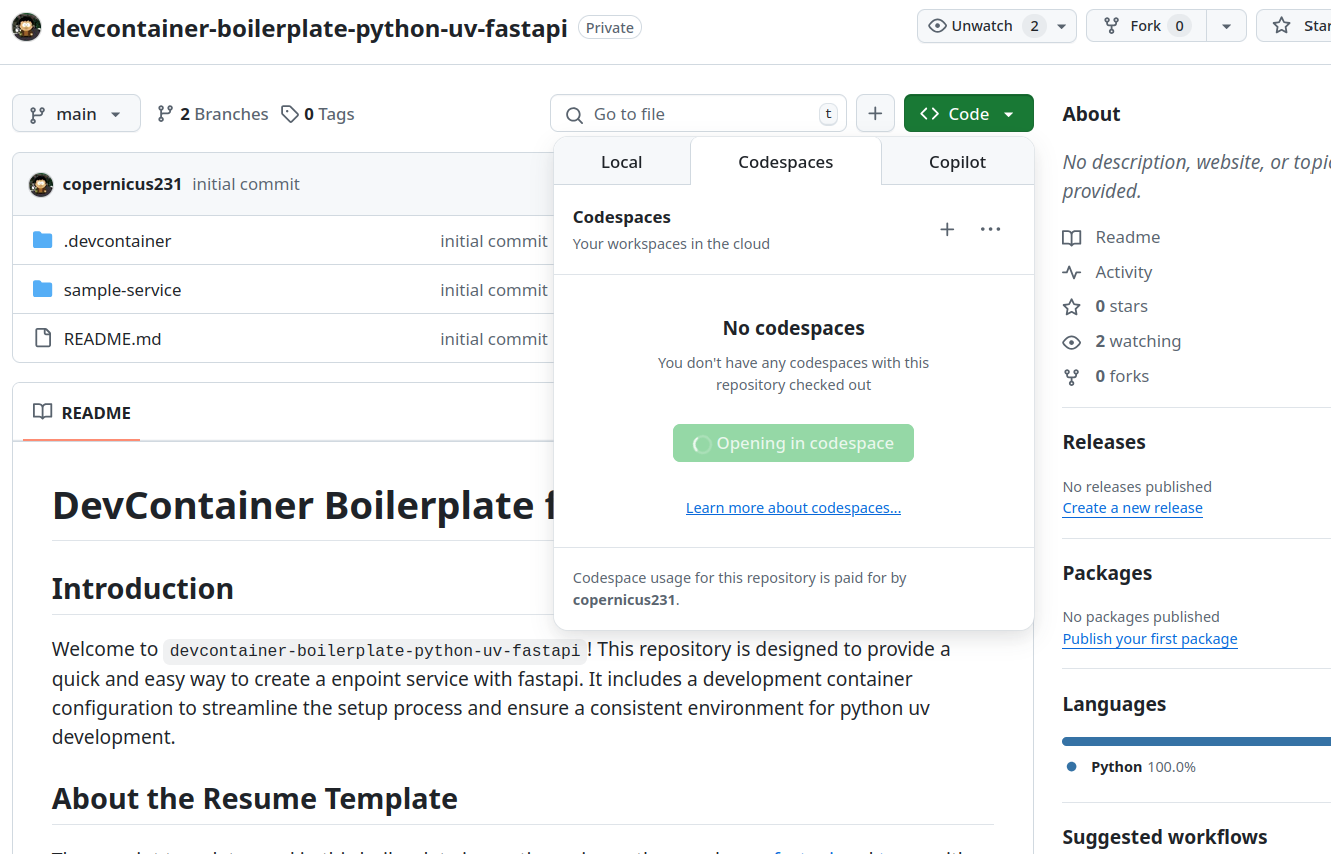
\includegraphics[width=\textwidth]{images/open-codespaces.png}
        \caption{Configuración de Codespaces.}
      \end{figure}
\end{frame}
\begin{frame}{Running codespaces}
  \begin{figure}
    \centering
    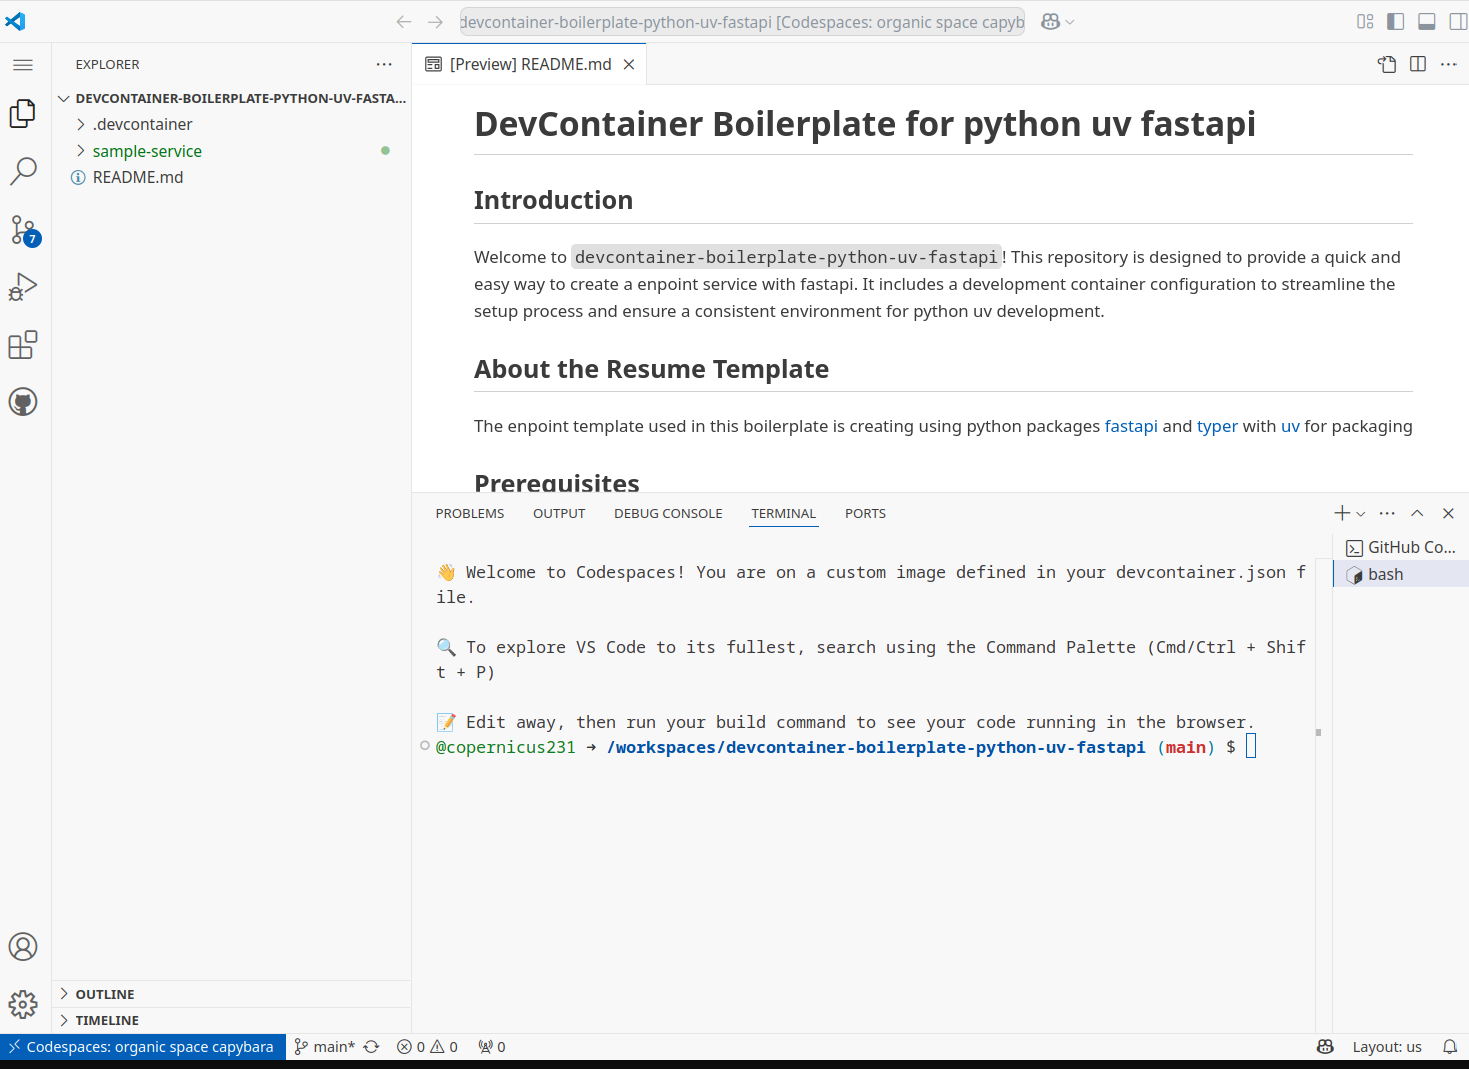
\includegraphics[width=\textwidth]{images/codespaces-up.png}
    \caption{Configuración de Codespaces.}
  \end{figure}
\end{frame}

\section{Archivos de configuracion}
\begin{frame}{Devcontainer Spec}
  El archivo de configuración permite describir cómo crear un contenedor y sus configuraciones de entorno, referencia en \href{https://containers.dev/implementors/json_reference/}{https://containers.dev/implementors/json\_reference/}
  \begin{block}{Archivo devcontainer.json}
    \begin{itemize}
      \item “devcontainer.json” dentro de la carpeta “.devcontainer”
      \item “.devcontainer.json”
      \item locaciones alternativas en sub carpetas de .devcontainer pueden ser definidas
    \end{itemize}
  \end{block}
\end{frame}
\subsection{Desafios asociados al desarollo en contenedores}
\subsection{Configuraciones basicas}
\begin{frame}{\subsecname}
  \lstinputlisting[language=json, firstline=2, lastline=4]{sample-config/devcontainer.json}
  \begin{block}{Base}
    \begin{itemize}
      \item \textbf{image:} Imagen base del contenedor.
      \item \textbf{name:} Nombre del contenedor.
      \item \textbf{containerUser:} Usuario dentro del contenedor.
    \end{itemize}
  \end{block}
\end{frame}
\begin{frame}{Features}
  Un feature es un stack a ser usado para el desarollo en este caso para desarollo en python
  \lstinputlisting[language=json, firstline=5, lastline=11]{sample-config/devcontainer.json}
  \begin{block}{Configuración de features}
    \begin{itemize}
      \item \textbf{common-utils:} Crea usuarios y configura la base del contenedor
      \item \textbf{uv:} Instala UV para manejar projectos python
      \\subsection{}item \textbf{python:} Instala python en este caso con la version 3.12
    \end{itemize}
  \end{block}
\end{frame}
\subsection{Customizaciones y extensiones}
\begin{frame}{\subsecname}
Cada IDE o ambiente puede tener customizaciones especificas y depende de cada provider que soporte devcotnainer implementarlas
\lstinputlisting[language=json, firstline=12, lastline=22]{sample-config/devcontainer.json}
\begin{block}{Configuración de extensiones}
  \begin{itemize}
    \item \textbf{extensions:} Lista de extensiones a instalar en el contenedor.
    \item \textbf{settings:} Configuraciones específicas del IDE.
  \end{itemize}
\end{block}
\end{frame}
\begin{frame}{Hooks de inicialización}
  \lstinputlisting[language=json, firstline=34, lastline=35]{sample-config/devcontainer.json}
  \begin{block}{Configuración de comandos}
    \begin{itemize}
      \item \textbf{postCreateCommand:} Comando a ejecutar después de crear el contenedor se ejecuta solo al momento de crear el contenedor.
      \item \textbf{initializeCommand:} Comando a ejecutar previa inicializacion del contenedor.
    \end{itemize}
  \end{block}
\end{frame}
\subsection{Otras configuraciones}
\begin{frame}{\subsecname}
  \lstinputlisting[language=json, firstline=23, lastline=33]{sample-config/devcontainer.json}
  \begin{block}{Configuración de otros parámetros}
    \begin{itemize}
      \item \textbf{containerEnv:} Environment variables a ser pasadas al contenedor.
      \item \textbf{mounts:} Montaje del volumen entre el host y el contenedor.
      \item \textbf{runArgs:} Argumentos a ser pasados a docker por ejemplo agregar gpus.
    \end{itemize}
  \end{block}
\end{frame}
\section{Ejemplos}
\subsection{Otros ejemplos de configuracion}
\begin{frame}{\subsecname}
  \begin{itemize}
    \small
    \item \textbf{TypeScript React.js+Nest.js:} \href{https://github.com/prulloac/devcontainer-boilerplate-typescript-vite-react-nest}{https://github.com/prulloac/devcontainer-boilerplate-typescript-vite-react-nest}
    \item \textbf{Python Flask:} \href{https://github.com/prulloac/devcontainer-boilerplate-python-poetry-flask}{https://github.com/prulloac/devcontainer-boilerplate-python-poetry-flask}
    \item \textbf{Java SpringBoot + TestContainer:} \href{https://github.com/prulloac/devcontainer-boilerplate-java-maven-springboot}{https://github.com/prulloac/devcontainer-boilerplate-java-maven-springboot}
    \item \textbf{Latex:} \href{https://github.com/prulloac/devcontainer-boilerplate-latex-resume}{https://github.com/prulloac/devcontainer-boilerplate-latex-resume}
    \item \textbf{Jupyter Notebook:} \href{https://github.com/prulloac/devcontainer-boilerplate-jupyter-poetry-langchain}{https://github.com/prulloac/devcontainer-boilerplate-jupyter-poetry-langchain}
    \item \textbf{Python+uv+FastAPI} \href{https://github.com/copernicus231/devcontainer-boilerplate-python-uv-fastapi}{https://github.com/copernicus231/devcontainer-boilerplate-python-uv-fastapi}
    \normalsize
  \end{itemize}
\end{frame}
\begin{frame}{Codespaces templates}
  \begin{figure}
    \centering
    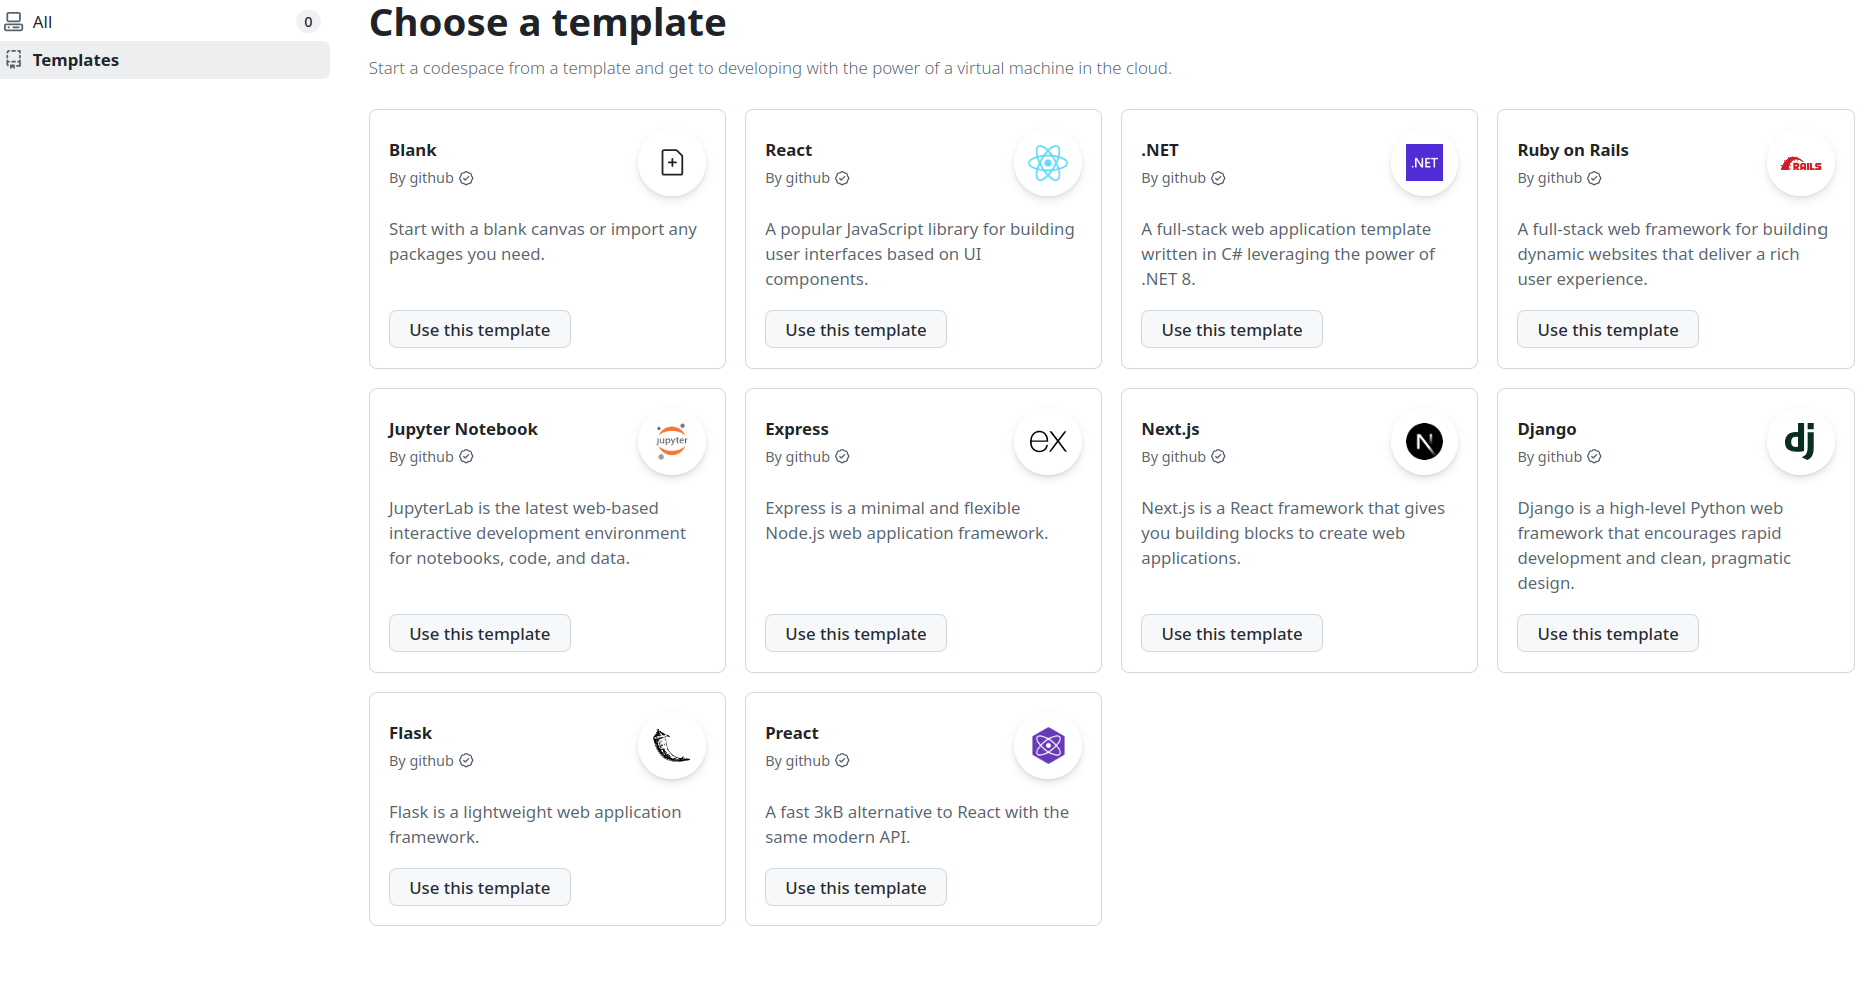
\includegraphics[width=\textwidth]{images/codespaces-templates.png}
    \caption{\href{https://github.com/codespaces/templates}{https://github.com/codespaces/templates}}
  \end{figure}
\end{frame}
\section{Conclusion}
\begin{frame}{Conclusion}
  \begin{itemize}
    \item \textbf{c1:} c1
    \item \textbf{c2:} c2
    \item \textbf{c3:} c3
  \end{itemize}
\end{frame}

\end{document}
